\documentclass[11pt]{article}

\usepackage[letterpaper,margin=1in]{geometry}
\usepackage[T1]{fontenc}
\usepackage{lmodern}
\usepackage{microtype}
\usepackage{amsmath,amssymb,amsthm,mathtools}
\usepackage{booktabs,tabularx,longtable,array}
\usepackage{graphicx}
\usepackage{float}
\usepackage[dvipsnames]{xcolor}
\usepackage{enumitem}
\usepackage[round,authoryear]{natbib}
\usepackage{xurl}
\usepackage{fancyhdr}
\usepackage{hyperref}
\usepackage[nameinlink,noabbrev]{cleveref}

\definecolor{Ink}{HTML}{17324D}
\definecolor{Accent}{HTML}{B43C4E}
\definecolor{Measured}{HTML}{8A5A16}
\hypersetup{
  colorlinks=true,
  linkcolor=Ink,
  citecolor=Ink,
  urlcolor=Accent,
  pdftitle={Reciprocal Tetration in the Logarithmic Lift},
  pdfauthor={Nick},
  pdfsubject={Reciprocal alternating exponentiation and lifted complex dynamics}
}

\pagestyle{fancy}
\fancyhf{}
\fancyhead[L]{\small Reciprocal tetration in the logarithmic lift}
\fancyhead[R]{\small Nick}
\fancyfoot[C]{\thepage}
\setlength{\headheight}{14pt}

\newtheorem{theorem}{Theorem}[section]
\newtheorem{proposition}[theorem]{Proposition}
\newtheorem{corollary}[theorem]{Corollary}
\newtheorem{lemma}[theorem]{Lemma}
\theoremstyle{definition}
\newtheorem{definition}[theorem]{Definition}
\newtheorem{observation}[theorem]{Computational observation}
\theoremstyle{remark}
\newtheorem{remark}[theorem]{Remark}

\newcommand{\C}{\mathbb C}
\newcommand{\R}{\mathbb R}
\newcommand{\Z}{\mathbb Z}
\newcommand{\Tet}{\operatorname{Tet}}
\newcommand{\Logp}{\operatorname{Log}}
\newcommand{\status}[1]{\textsf{\textbf{#1}}}
\newcommand{\e}{\mathrm e}

\title{\bfseries Reciprocal Tetration in the Logarithmic Lift\\[0.35em]
\large Fixed pairs, periodic sign weaves, and branch-sensitive dynamics}
\author{Nick\\\small Independent Researcher}
\date{Research preprint v1.0 -- August 12, 2026}

\begin{document}
\maketitle

\begin{abstract}
We begin with the finite, right-associated height-$n$ power tower and retain both phases of an alternating tower.  Fixing the second visible base to be the reciprocal of the first, $b=a^{-1}$, and writing $a=\e^L$ gives the one-complex-parameter map
\[
  F_L(P,M)=\bigl(\e^{LM},\e^{-LP}\bigr).
\]
This paper develops the exact foundation of that lifted family.  Positive-real fixed pairs satisfy $P\log P+M\log M=0$, admit a global one-variable chart, and attract the cap-$1$ alternating tower for every real $L$.  Two pair updates decouple into the scalar entire maps $g_L(z)=\exp(L\exp(-Lz))$ and $g_{-L}$.  More generally, if $b=a^c$, $L=\e^\kappa$, and $c=\e^\delta$, the two-base scalar return is affinely conjugate to $E_\kappa\circ E_{\kappa+\delta}$, where $E_\kappa(z)=\e^z+\kappa$.  The autonomous one-base return and the reciprocal return are therefore the $c=1$ and $c=-1$ slices of the same family.  The $c=-1$ centerline return, its convergence boundary and multiplier bookkeeping, and its antiholomorphic half-step already occur in \citet{BakerRippon1989Composite}.  We retain the ordered reciprocal pair and develop its exact Dottie identification, branch-aware fixed data, periodic sign weaves, and cap-selected certified anchors.  Finite-resolution surveys display a reversal-order effect and a structured complex $L$-plane, while directed ball arithmetic isolates a paired period-$640$ Dottie anchor and a paired period-$190$ off-axis anchor called Sirius.  Exact, certified, measured, conditional, and open statements are separated throughout.
\end{abstract}

\noindent\textbf{Keywords.} tetration; iterated exponentiation; cyclic exponentials; Lambert $W$; complex dynamics; interval arithmetic.\\
\textbf{MSC 2020.} 30D05, 37F10, 37F46, 65G30.

\medskip
\noindent\fcolorbox{Ink}{Ink!4}{\parbox{0.955\linewidth}{\small
\textbf{Evidence convention.} \status{Exact} denotes an algebraic or analytic consequence of the displayed definitions or a cited theorem.  \status{Certified} denotes a directed outward-rounded enclosure tied to a retained proof record.  \status{Measured} denotes finite arbitrary-precision or raster evidence.  \status{Conditional} states all required hypotheses.  \status{Open} marks a question for which no conclusion is claimed.  Dark or unresolved atlas pixels are computation horizons, not assertions of divergence.}}

\section{Introduction and scope}

Alternating and cyclic positive-base towers are classical; see \citet{CreutzSternheimer1981}, \citet{BakerRippon1985,BakerRippon1989,BakerRippon1989Composite}, and \citet{Bulanov2001,Bulanov2010}.  We study the fixed reciprocal specialization
\[
  b=a^{-1},\qquad a=\e^L,\qquad b=\e^{-L},
\]
retain the ordered phase pair, and take the logarithmic lift $L$ rather than the visible base $a$ as the parameter.  The lift is essential in complex dynamics: $L$ and $L+2\pi i k$ represent the same visible base, and their first cap iterate agrees, but subsequent iterates generally differ.

Throughout, $\Logp z$ is the principal logarithm with $\arg z\in(-\pi,\pi]$, and $\log_k z=\Logp z+2\pi i k$.  At a branch cut, the continuation side is additional retained data.  For later orientation, let $d\in(0,\pi/2)$ solve $d=\cos d$ and put
\begin{equation}
  L_*=i\exp(-\sin d).
  \label{eq:dottie-Lstar}
\end{equation}
This location is classical prior art.  Theorem~8.1 of \citet{BakerRippon1989Composite} gives the alternating-conjugate boundary
\[
  \mathcal C=\{\sigma\e^{-\bar\sigma}:|\sigma|\le1\};
\]
putting $\sigma=\sin d+id$ gives $|\sigma|=1$ and $\sigma\e^{-\bar\sigma}=L_*$.  The companion paper \citep{NickDottie2026} identifies their boundary data exactly with the Dottie number and develops the subsequent local and cap-marked dynamics.

For this reciprocal lifted family, this paper develops the fixed-pair chart, branch-sensitive complex parametrizations, phase-aware sign-word formulation, and a reproducibility discipline that turns selected pixels into orbit statements.  The surrounding theories of cyclic exponentiation, Lambert $W$, finite-type entire maps, and interval arithmetic remain those of the cited literature.  The exact Dottie identity and spire geometry are treated in the companion paper.

The standard complex exponential family $E_\kappa(z)=\e^z+\kappa$ treats a complex state and an additive parameter \citep{RempeSchleicher2008}.  The correct comparison with alternating tetration uses the common two-base family $b=a^c$.  In the coordinates of \cref{prop:one-phase-slice}, the equal-base return is the $c=1$ slice $E_\kappa^2$, while the reciprocal return is the $c=-1$ slice $E_\kappa\circ E_{\kappa+\pi i}$.  Positive aligned two-base cases lie at $c>0$; alternating-conjugate coefficients satisfy $|c|=1$ and include $c=-1$ on the imaginary axis; the cited Bulanov regime lies at $|c|>1$ \citep{BakerRippon1985,BakerRippon1989Composite,Bulanov2001}.  Our scope is the retained ordered $c=-1$ pair, its cap and branch data, and the structures developed after the exact Dottie identification.

There is a useful distinction from the signed-tower problem of \citet{MazetHalberstadt2025}.  Their maps are $x\mapsto \pm \e^{cx}$, with the sign outside the exponential.  Here
\[
  X_j=\exp(s_jL X_{j+1}),\qquad s_j\in\{+1,-1\},
\]
puts the sign inside the exponent and selects the reciprocal base $\e^{s_jL}$.  The two settings are adjacent but not identical.

\section{Finite Tet and the reciprocal pair}

\begin{definition}[Finite Tet function]
For $L\in\C$, cap $1$, and integer $n\ge0$, define
\begin{equation}
  \Tet_L(0;1)=1,
  \qquad
  \Tet_L(n+1;1)=\exp\!\bigl(L\Tet_L(n;1)\bigr).
  \label{eq:finite-tet}
\end{equation}
For a positive real base $a$ on its real lift $L=\log a$, this is the usual right-associated finite power tower.
\end{definition}

For example, $\Tet_{\log 1.25}(5;1)$ contains five copies of $1.25$:
\[
  1.25^{\,1.25^{\,1.25^{\,1.25^{\,1.25}}}}.
\]
An infinite tower, when it exists, is a limit of finite towers.  No infinite-height value is built into \cref{eq:finite-tet}.

Alternating the bases $\e^L$ and $\e^{-L}$ produces two outer phases.  Rather than identify them in one scalar expression, update them simultaneously:
\begin{equation}
  P_{n+1}=\e^{LM_n},\qquad
  M_{n+1}=\e^{-LP_n},
  \qquad (P_0,M_0)=(1,1).
  \label{eq:pair-recurrence}
\end{equation}

\begin{definition}[Reciprocal Tet pair map]
For $L\in\C$, let
\begin{equation}
  F_L(P,M)=\bigl(\e^{LM},\e^{-LP}\bigr).
  \label{eq:pair-map}
\end{equation}
A fixed point of $F_L$ is a reciprocal Tet pair at lift $L$.
\end{definition}

The ordered pair is part of the output.  Its entries exchange under $L\mapsto-L$ and can lie on different scalar basins even when a single marked probe looks stationary.

\section{Exact positive-real fixed-pair algebra}

Suppose $L,P,M\in\R$ and $P,M>0$.  At a fixed pair,
\begin{equation}
  P=\e^{LM},\qquad M=\e^{-LP}.
  \label{eq:real-fixed}
\end{equation}

\begin{proposition}[Compatibility and recovery]\label{prop:real-compat}
Every positive-real reciprocal fixed pair satisfies
\begin{equation}
  P\log P+M\log M=0,
  \qquad P^P M^M=1.
  \label{eq:compatibility}
\end{equation}
The lift and visible base are recovered by
\begin{equation}
  L=\frac{\log P}{M}=-\frac{\log M}{P},
  \qquad a=P^{1/M}=M^{-1/P}.
  \label{eq:recovery}
\end{equation}
\end{proposition}

\begin{proof}
Take real logarithms in \cref{eq:real-fixed}, multiply the first relation by $P$ and the second by $M$, and add.  Solving the same logarithmic equations for $L$ and $a$ gives \cref{eq:recovery}.
\end{proof}

Put $U=\log P$, $V=\log M$, and $q=U-V$.  Then $U=L\e^V$ and $V=-L\e^U$.

\begin{proposition}[Global real chart]\label{prop:q-chart}
The positive-real fixed-pair locus is parametrized by $q\in\R$ as
\begin{align}
  U(q)&=\frac{q}{1+\e^q},
  &V(q)&=-\frac{q\e^q}{1+\e^q},\label{eq:uv-chart}\\
  P(q)&=\e^{U(q)},
  &M(q)&=\e^{V(q)},\label{eq:pm-chart}\\
  L(q)&=\frac{q}{P(q)+M(q)}.\label{eq:l-chart}
\end{align}
The involution $q\mapsto-q$ swaps $P$ and $M$ and sends $L$ to $-L$.
\end{proposition}

\begin{proof}
Since $q=U-V=L(M+P)$, \cref{eq:l-chart} follows.  For $q\ne0$ (equivalently $L\ne0$), dividing $U=L\e^V$ by $-V=L\e^U$ gives $U/(-V)=\e^{V-U}=\e^{-q}$; solving together with $U-V=q$ yields \cref{eq:uv-chart}.  At $q=0$, the fixed equations with $U=V$ force $U=V=0$, and the formulas follow directly (or by continuity).  The remaining statements are direct substitutions.

For $q>0$, one may write
\[
  L(q)=\frac{q\e^{-U(q)}}{1+\e^{-q}},
  \qquad
  \frac{d}{dq}\log L(q)=\frac1q+\frac{q\e^q}{(1+\e^q)^2}>0.
\]
Oddness handles $q<0$, while $L'(0)=1/2$ and $L(q)\sim q$ as $q\to+\infty$.  Hence $q\mapsto L(q)$ is a bijection from $\R$ onto $\R$.
\end{proof}

\begin{corollary}[Convergence on the full real reciprocal slice]\label{cor:real-convergence}
For every real lift $L$, the cap-$1$ reciprocal orbit \cref{eq:pair-recurrence} converges to the unique positive-real fixed pair in \cref{prop:q-chart}.
\end{corollary}

\begin{proof}
In the notation of the Baker--Rippon criterion, $\log a=U\e^{-V}$ and $\log b=V\e^{-U}$, while
\[
  |UV|=\frac{q^2\e^q}{(1+\e^q)^2}
       =\frac{q^2}{4\cosh^2(q/2)}<1.
\]
The chart $L(q)$ is odd, strictly increasing, and onto $\R$.  The unnumbered theorem of \citet{BakerRippon1985} therefore gives convergence for every real $L$; uniqueness of the positive-real fixed pair is already contained in \cref{prop:q-chart}.
\end{proof}

The individual coordinates have a sharp maximum.  If $P>1$ and $0<M<1$, \cref{eq:compatibility} gives $P\log P=-M\log M$.  The right-hand side is maximized at $M=\e^{-1}$.

\begin{corollary}[Coordinate maximum]
\begin{equation}
  P_{\max}=\exp W_0(1/\e)
  =1.3210997620156174569\ldots.
  \label{eq:pmax}
\end{equation}
Here $W_0$ denotes the principal Lambert-$W$ branch \citep{CorlessEtAl1996}.
It occurs at
\begin{align}
  L_c&=\e\,W_0(1/\e)=\e^{-W_0(1/\e)}
       =0.7569451064575836646\ldots,\notag\\
  a_c&=\e^{L_c}=2.1317539817238058\ldots.
\end{align}
The lift itself is unbounded along the real chart; $L_c$ locates the coordinate maximum, not a maximum of $L$.
\end{corollary}

\begin{proof}
At the maximum $M=\e^{-1}$.  With $w=\log P$, compatibility gives $w\e^w=1/\e$, hence $w=W_0(1/\e)$ and $P=\e^w$.  Recovery gives $L=\log P/M=\e w=\e^{-w}$.
\end{proof}

\begin{figure}[t]
  \centering
  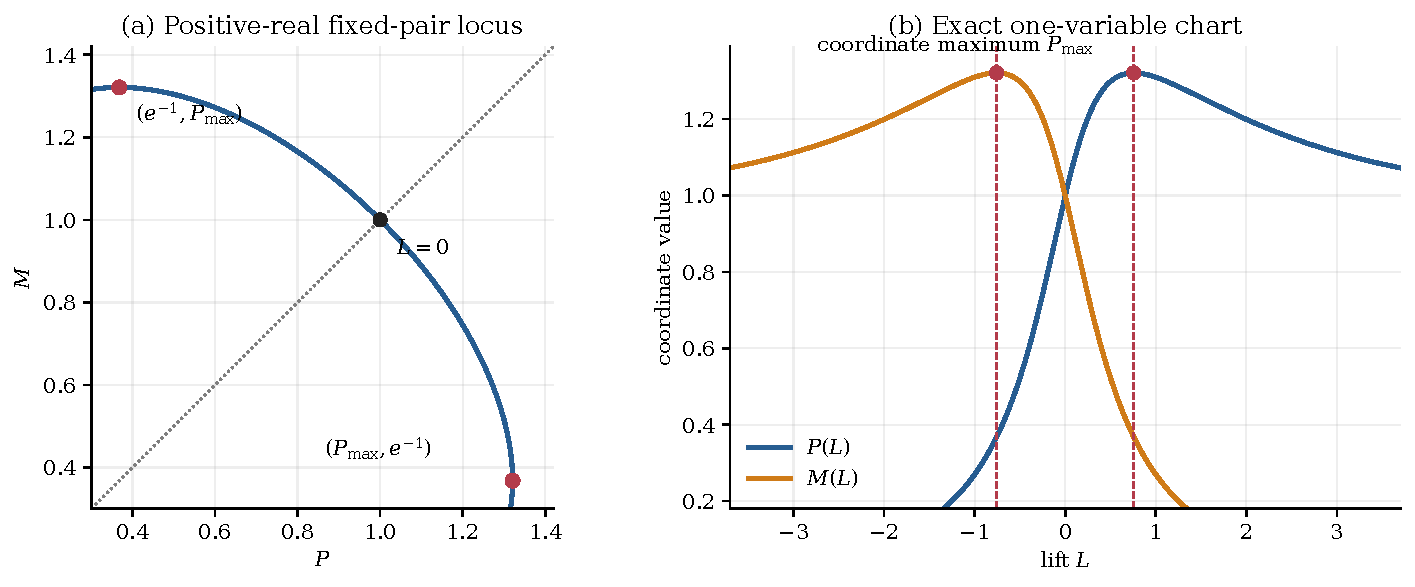
\includegraphics[width=\textwidth]{figures/real_fixed_pair_chart.pdf}
  \caption{The exact positive-real fixed-pair locus and its global $L$-chart.  The red points mark the maxima of the individual coordinates; the lift continues beyond them without bound.}
  \label{fig:real-chart}
\end{figure}

\section{Two-step scalar reduction and marked values}

\begin{proposition}[Scalar decoupling]\label{prop:decoupling}
Define
\begin{equation}
  g_L(z)=\exp\!\bigl(L\exp(-Lz)\bigr).
  \label{eq:gL}
\end{equation}
Then
\begin{equation}
  F_L^2(P,M)=\bigl(g_L(P),g_{-L}(M)\bigr).
  \label{eq:two-step}
\end{equation}
\end{proposition}

\begin{proposition}[Two-base family and reciprocal slice]\label{prop:one-phase-slice}
Let
\[
  E_\kappa(u)=\e^u+\kappa.
\]
For $L,c\ne0$, choose $\kappa,\delta\in\C$ with $\e^\kappa=L$ and $\e^\delta=c$, and put
\[
  g_{L,c}(z)=\exp\!\bigl(L\exp(cLz)\bigr),
  \qquad
  C_{\kappa,c}(z)=\kappa+cLz.
\]
Then
\begin{equation}
  C_{\kappa,c}\circ g_{L,c}\circ C_{\kappa,c}^{-1}
  =E_\kappa\circ E_{\kappa+\delta}.
  \label{eq:one-phase-slice}
\end{equation}
For $c=1$, this is the equal-base return and the right side is $E_\kappa^2$.  For $c=-1$, choose $\delta=\pi i$; then $g_{L,-1}=g_L$, $C_{\kappa,-1}(z)=\kappa-Lz$, and the right side is $E_\kappa\circ E_{\kappa+\pi i}$.  Consequently, $z_{n+1}=g_{L,c}(z_n)$ is equivalent under $u_n=C_{\kappa,c}(z_n)$ to the alternating orbit
\[
  u_n\xmapsto{E_{\kappa+\delta}}v_n
  \xmapsto{E_\kappa}u_{n+1}.
\]
The coordinates realign after every two exponential stages, and a primitive period-$p$ orbit of $g_L$ becomes a phase-labelled alternating orbit of $2p$ stages.
\end{proposition}

\begin{proof}
Direct composition gives
\[
  E_\kappa\!\left(E_{\kappa+\delta}(u)\right)
  =\kappa+cL\exp(\e^u).
\]
Also $C_{\kappa,c}^{-1}(u)=(u-\kappa)/(cL)$, so
\[
  C_{\kappa,c}\!\left(g_{L,c}(C_{\kappa,c}^{-1}(u))\right)
  =\kappa+cL\exp(\e^u).
\]
This proves \cref{eq:one-phase-slice}; the orbit statement follows by iteration.
\end{proof}

Thus $E_\kappa^2$ is not a slice of $E_\kappa\circ E_{\kappa+\pi i}$: they are the $c=1$ and $c=-1$ slices of the common family in \cref{eq:one-phase-slice}.  In Theorem~8.1 of \citet{BakerRippon1989Composite}, alternating-conjugate coefficients have $c=\bar L/L$, hence $|c|=1$; on $L=iy$ this is exactly $c=-1$.  The reciprocal scalar return and its centerline half-step therefore have a direct predecessor.  What is retained here beyond that predecessor is the simultaneous ordered pair, its two marked scalar values, logarithmic branch witnesses, cap selection, and the later Dottie/Spire orbit geometry.

For $L=0$, $g_0\equiv1$.  Assume henceforth in this paragraph that $L\ne0$.  The derivative
\begin{equation}
  g_L'(z)=-L^2\e^{-Lz}g_L(z)
  \label{eq:g-derivative}
\end{equation}
never vanishes when $L\ne0$.  Let $\operatorname{Sing}(f^{-1})$ denote the finite singular values of an entire function $f$.  For $A_L(z)=\e^{Lz}$ and $B_L(z)=\e^{-Lz}$,
\[
  \operatorname{Sing}((A_L\circ B_L)^{-1})
  \subseteq \operatorname{Sing}(A_L^{-1})
  \cup A_L\!\left(\operatorname{Sing}(B_L^{-1})\right)
  =\{0,1\};
\]
both values are attained asymptotically.  Indeed, $z=t/L$ gives $g_L(z)\to1$ as $t\to+\infty$.  Choosing a continuous logarithm along the curve $
\e^{-Lz}=-t/L$, equivalently
$z=-L^{-1}\log(-t/L)$, gives $g_L(z)=\e^{-t}\to0$.  There are no critical values.  Hence $\operatorname{Sing}(g_L^{-1})=\{0,1\}$, and $g_L$ is a finite-type entire map in the sense of \citet{EremenkoLyubich1992}.  The first pair coordinate interleaves their marked orbits:
\begin{equation}
  P_{2n}=g_L^n(1),
  \qquad
  P_{2n+1}=g_L^{n+1}(0).
  \label{eq:marked-interleave}
\end{equation}
Thus cap portraits are organized by both marked values even when only one seed is displayed.

Let $S(P,M)=(M,P)$ and $K(P,M)=(\overline P,\overline M)$.  Direct substitution gives
\begin{equation}
  F_{-L}=S\circ F_L\circ S,
  \qquad
  F_{\overline L}=K\circ F_L\circ K.
  \label{eq:pair-symmetries}
\end{equation}
Since both involutions fix $(1,1)$, the cap dynamics have the corresponding fourfold symmetry.  This does not create a vertical translation symmetry in the $L$-plane.

If $A_L(z)=\e^{Lz}$ and $B_L(z)=\e^{-Lz}$, then
\begin{equation}
  g_L=A_L\circ B_L,
  \qquad g_{-L}=B_L\circ A_L,
\end{equation}
with semiconjugacies
\[
  B_L\circ g_L=g_{-L}\circ B_L,
  \qquad
  A_L\circ g_{-L}=g_L\circ A_L.
\]
For $L\ne0$, $A_L$ and $B_L$ induce mutually inverse bijections on cyclic periodic orbits of the two scalar factors, inverse up to one cyclic shift, preserving primitive period and cycle multiplier.  They need not send the same marked seed into corresponding basins.

At integer imaginary lifts there is an exact landing family.  For $k\in\Z\setminus\{0\}$, $L=k\pi i$, and $\sigma=(-1)^k$,
\begin{equation}
  g_L(0)=g_L(1)=g_L(\sigma)=\sigma,
  \qquad g_L'(\sigma)=k^2\pi^2.
\end{equation}
The ordered pair cap maps from $(1,1)$ to $(\sigma,\sigma)$ in exactly one pair update, and the scalar cap lands on the same repelling fixed state after one scalar update.

The following atlas is a historical finite numerical classification retained for orientation.  Its raw two-dimensional arrays do not survive, so no pixel is promoted beyond the metadata printed in the caption.  Every retained run stayed in $|\operatorname{Im}L|\le\pi$; this strip is not a dynamical fundamental domain, $L\mapsto L+2\pi i k$ is not a symmetry of the lifted family, and no behavior is extrapolated across the plotted boundary.

\begin{figure}[t]
  \centering
  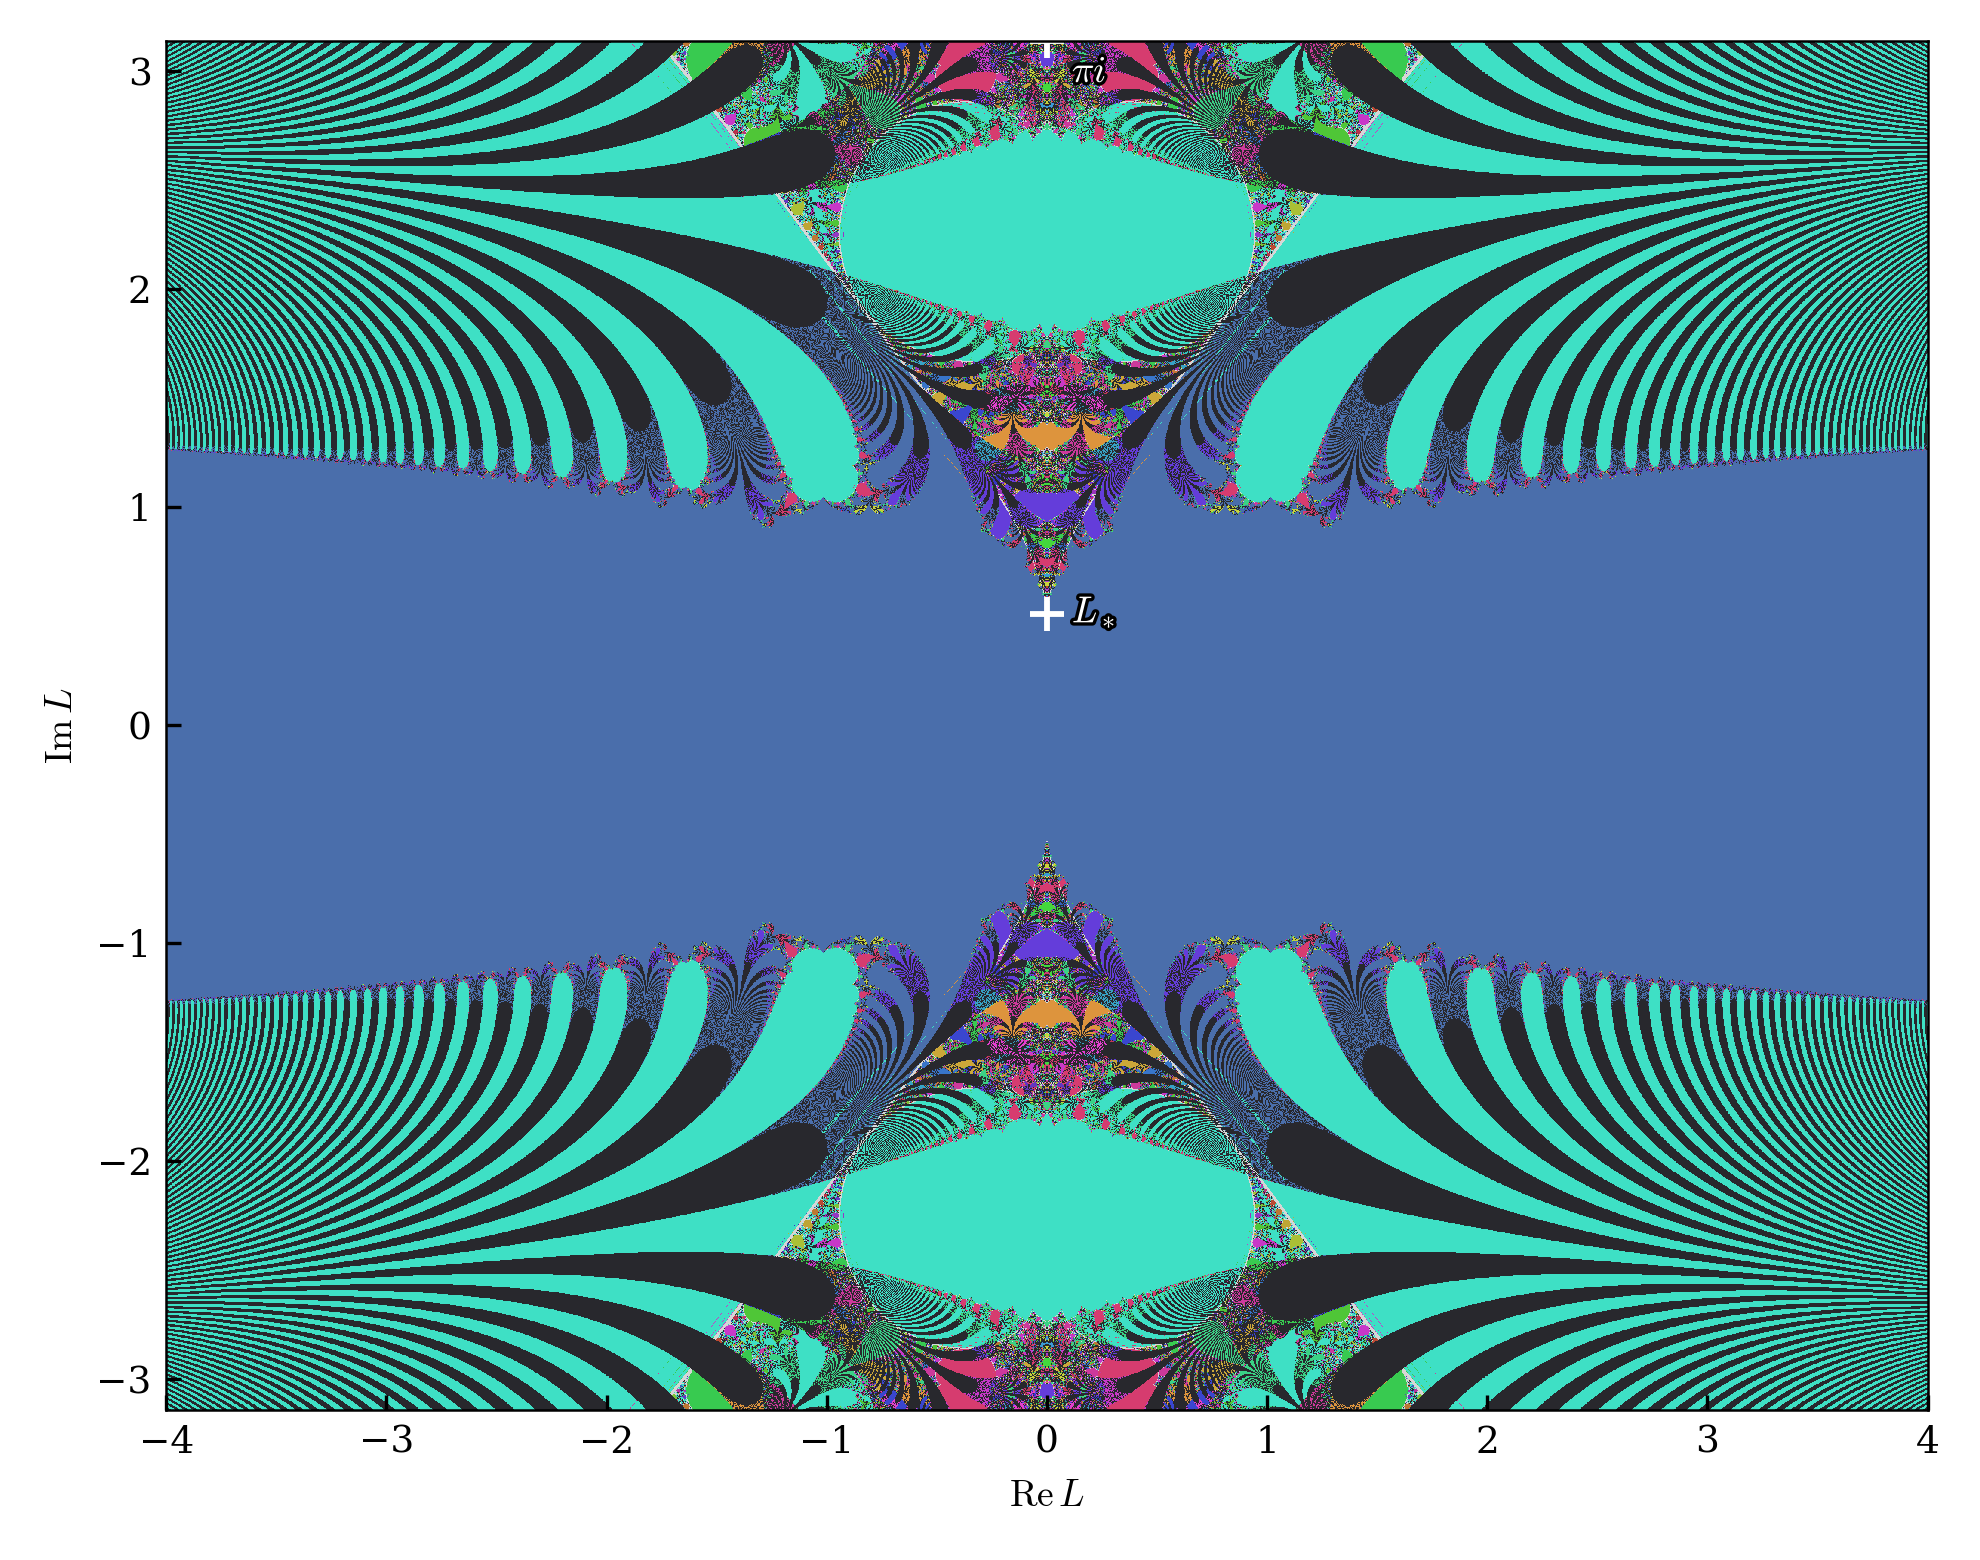
\includegraphics[width=\textwidth]{figures/complex_lift_atlas.png}
  \caption{\status{Measured.} A $4097\times3217$ cap-orbit atlas over $\operatorname{Re}L\in[-4,4]$ and $\operatorname{Im}L\in[-\pi,\pi]$, using at most $8000$ pair updates, candidate paired periods $p_{\rm pair}\le128$, and FP64 tolerance $10^{-11}$.  Colors encode measured classes.  Blue, gray, and dark regions include arithmetic and iteration horizons.  The marked point $L_*$ is the exact Dottie parameter developed in the companion paper.}
  \label{fig:atlas}
\end{figure}

\section{Branch-sensitive complex fixed data}

Complex logarithms must be retained as witnesses.  Write
\begin{equation}
  \log_{k_P}P=LM,
  \qquad
  \log_{k_M}M=-LP,
  \qquad
  P\log_{k_P}P+M\log_{k_M}M=0,
  \label{eq:complex-compatibility}
\end{equation}
for specified logarithmic continuation sides.  Equivalently, put
\begin{equation}
  U=LM,\qquad V=-LP,\qquad P=\e^U,\qquad M=\e^V.
\end{equation}
At a fixed pair,
\begin{equation}
  U\e^U+V\e^V=0.
  \label{eq:lambert-balance}
\end{equation}

\begin{proposition}[Lambert-$W$ atlas]\label{prop:lambert-atlas}
Let $x\ne0$ and choose branches $k,m\in\Z$ such that
\begin{equation}
  U=W_k(x),\qquad V=W_m(-x).
\end{equation}
Then, on the specified continuation sides,
\begin{equation}
  L=-\frac{UV}{x},
  \qquad P=\e^U,
  \qquad M=\e^V
  \label{eq:lambert-atlas}
\end{equation}
is fixed data for $F_L$.  Conversely, every fixed pair with $L\ne0$ determines such $x,U,V$ and branch witnesses.  Its scalar multiplier is
\begin{equation}
  g_L'(P)=UV.
\end{equation}
\end{proposition}

\begin{proof}
Set $x=U\e^U=-V\e^V$.  Then $U=W_k(x)$ and $V=W_m(-x)$ on suitable inverse branches.  Since $x=UP$, the identity $L=-UV/x=-V/P$ recovers $V=-LP$; similarly $U=LM$.  Finally, \cref{eq:g-derivative} at a fixed point gives $g_L'(P)=-L^2PM=UV$.
\end{proof}

The branch structure of $W$ is as in \citet{CorlessEtAl1996}.  Integer branch labels alone do not encode which side of a cut a continuation uses; a complete orbit record must preserve continuation and sheet information.

\section{Periodic reciprocal sign words}

This is the reciprocal-alphabet specialization of cyclic exponentiation; compare \citet{BakerRippon1989,Bulanov2010}.

Let
\[
  w=(s_0,\ldots,s_{r-1}),\qquad s_j\in\{+1,-1\}.
\]
The $r$-phase reciprocal weave is
\begin{equation}
  X_{j,n+1}=\exp(s_jL X_{j+1,n}),
  \qquad j\pmod r,
  \qquad X_{j,0}=1.
  \label{eq:sign-word}
\end{equation}
The reciprocal pair is the word $(+,-)$.  A limiting phase tuple satisfies $X_j=\e^{s_jLX_{j+1}}$, and each edge recovers the same lift after a sheet integer $k_j$ is chosen:
\begin{equation}
  L=\frac{\Logp X_j+2\pi i k_j}{s_jX_{j+1}}.
  \label{eq:edge-recovery}
\end{equation}

Three operations organize the word space:
\begin{equation}
  (Rw)_j=s_{j+1},\qquad
  (Vw)_j=s_{-j},\qquad
  (Cw)_j=-s_j,
  \qquad j\pmod r,
  \label{eq:RVC}
\end{equation}
where $R,V,C$ denote rotation, reversal, and complement.  Consequently:
\begin{enumerate}[label=(\roman*),leftmargin=2em]
  \item rotation relabels phases;
  \item global sign complementation corresponds to $L\mapsto-L$;
  \item reversal changes the order of a directed exponential composition.
\end{enumerate}
For the two letters, $A_L\circ B_L$ and $B_L\circ A_L$ are generically unequal.  Order sensitivity is present in the defining algebra before any raster is drawn.  Rotations and reversal generate a dihedral action, while complement commutes with both.  Words with nontrivial stabilizers produce Schreier quotients of the generic action graph.

\begin{observation}[Reversal-order effect]\label{obs:chirality}
\status{Measured.} In an archived $385\times303$ sign-word survey on $[-4,4]\times[-\pi,\pi]$, cap $X_{j,0}=1$, $3072$ simultaneous tuple updates, and tuple-period cap $96$, four non-self-reversal pairs with equal length and sign count disagreed on approximately $14.784\%$, $13.035\%$, $11.962\%$, and $2.155\%$ of grid tuple-period codes.  Of $208$ representatives replayed at $80$ digits for $12000$ tuple updates, $168$ retained the proposed tuple period, four were reclassified, and $36$ remained beyond the precision or iteration horizon.
\end{observation}

This establishes a robust finite-resolution order effect.  It is not yet a conjugacy-invariant chirality theorem.

\noindent\emph{Measured record.}  The retained summary, reversal comparison, arbitrary-precision replay JSON, catalog, metrics, and survey/probe scripts are frozen under \path{reproducibility/records/legacy_sign_word_survey/}.  The broad complex-atlas raw arrays do not survive and are not reconstructed from the rendered figure.

\begin{figure}[t]
  \centering
  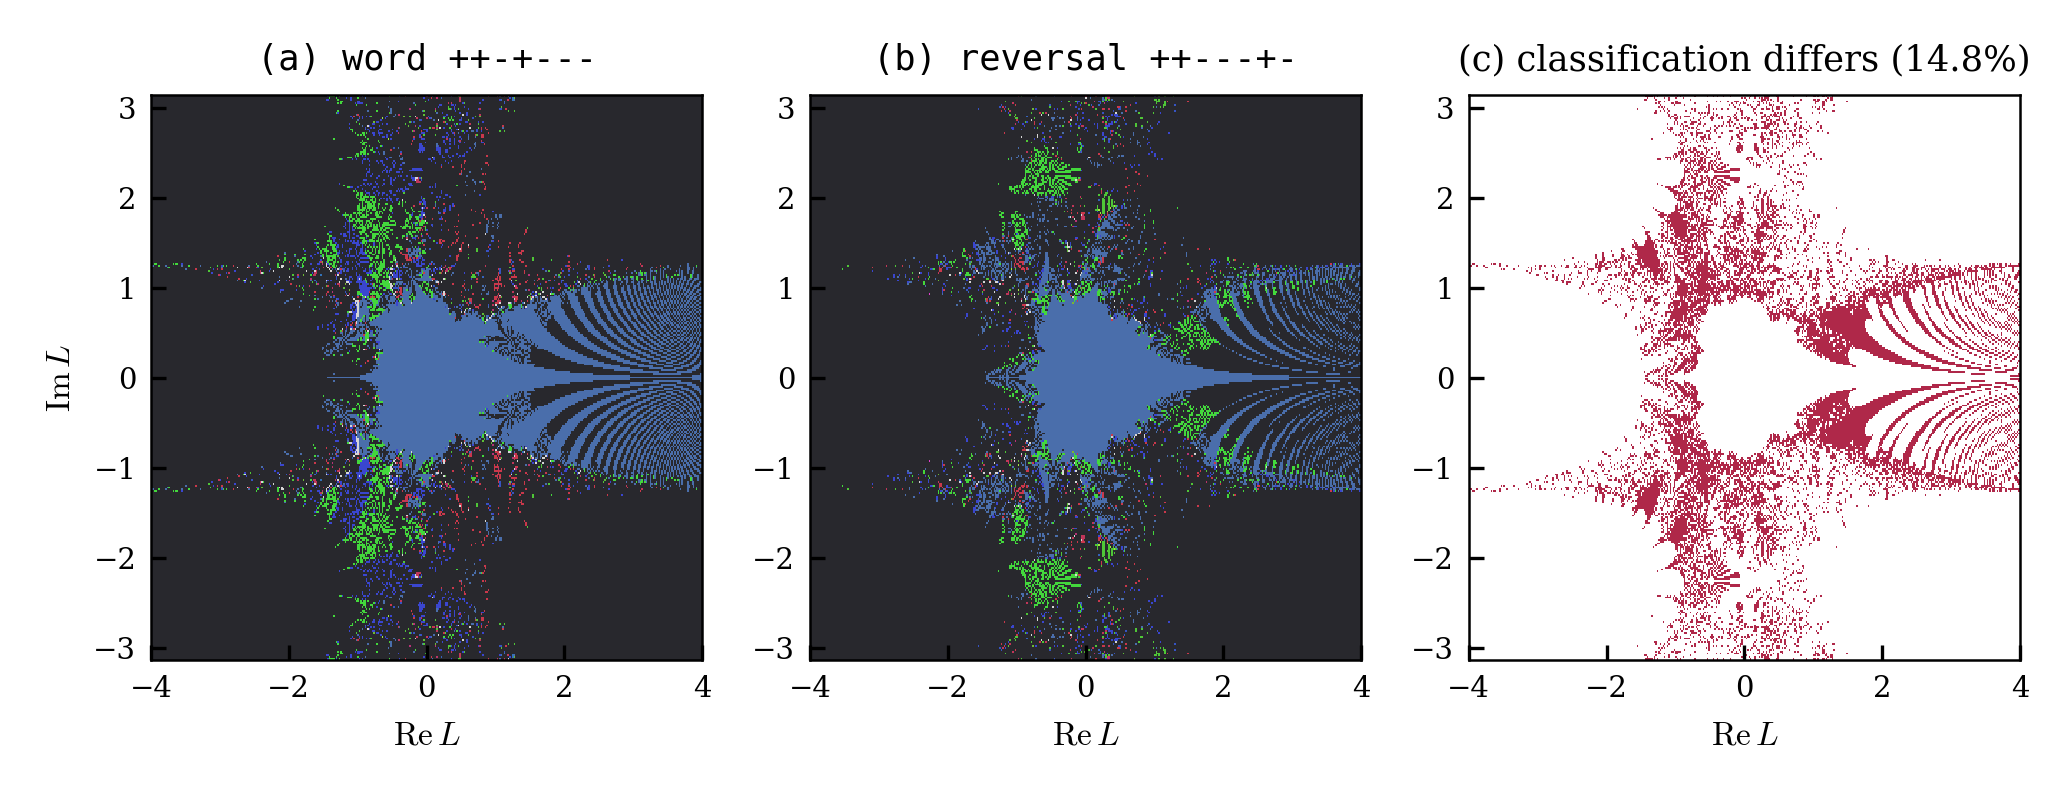
\includegraphics[width=\textwidth]{figures/reversal_order_effect.png}
  \caption{\status{Measured.} A length-seven sign word, its reversal, and the pixels where their finite tuple-period classifiers differ.  Primitive words, rather than padded repetitions, are the natural catalog entries.}
  \label{fig:reversal}
\end{figure}

Period reporting must name its clock.  If $T_w$ denotes one simultaneous tuple update for a length-$r$ word, then one complete word block is $T_w^r$.  Thus a tuple orbit of least $T_w$-period $q$ has word-block period $q/\gcd(q,r)$; a selected coordinate period can differ as well.  This bookkeeping becomes essential for the Dottie even/odd split.

\section{Orbit branch grammar}

For a scalar edge $z_{j+1}=g_L(z_j)$, put
\begin{equation}
  \Lambda_j=\Logp z_{j+1}+2\pi i k_j.
\end{equation}
When $z_j\ne0$, the equation $\Lambda_j=L\e^{-Lz_j}$ gives
\begin{equation}
  L=-\frac{W_{m_j}(-z_j\Lambda_j)}{z_j},
  \qquad (k_j,m_j)\in\Z^2.
  \label{eq:edge-address}
\end{equation}
The pair $(k_j,m_j)$ is an edge address.  A periodic orbit produces a cyclic address word; every phase must reconstruct the same $L$ through \cref{eq:edge-address}.  The spread of those reconstructions is a stringent common-parameter checksum.  At the marked edge $z_j=0$, division is avoided:
\[
  z_{j+1}=\e^L,
  \qquad L=\Logp z_{j+1}+2\pi i k_j.
\]

For a branch-addressed promotion, a colored pixel should be replaced by a closure equation, proper-divisor exclusions, a multiplier, a cyclic access word, and repeated reconstruction of one common lift.  A forward proof may instead use independent trapping disks and directed cap capture, as in the next section.

\section{Directed anchors in the lifted plane}

The computer-assisted propositions in this section use midpoint-radius Arb/ACB balls and directed trapping-disk arguments; see \citet{MooreKearfottCloud2009,Johansson2017,Rump2010}.  The same reference implementation was rerun at $256$ and $512$ bits, with a separate gate/test harness and manifest verifier.  Uniqueness is local to the declared disks.  The source, exact rational inputs, result JSON, tests, and hashes are frozen in computational supplement v1.0.  Its index assigns the short record identifiers \texttt{P3A-D640} and \texttt{P3A-S190}; the supplement should receive a persistent identifier upon submission.

\subsection{A marked Dottie-ladder orbit}

At the exact rational centerline value
\begin{equation}
  y=\frac{50989298353866910770690528562065021598851444975750428168910979807}{10^{65}},
  \qquad L=iy,
  \label{eq:p640-rational}
\end{equation}
the exact disk $D$ of radius $10^{-14}$ centered at the rational phase in record \texttt{P3A-D640} contains $z=1$ strictly and is mapped strictly into itself by $g_L^{320}$.

\begin{proposition}[Certified paired period $640$ anchor]\label{prop:p640}
At \cref{eq:p640-rational},
\[
  \sup_{z\in D}|(g_L^{320})'(z)|
  <6.35078306256\times10^{-17}.
\]
All proper divisors of $320$ are excluded, with minimum separation above $0.57419$.  The conjugate product disk is strictly invariant and contracting under $F_L^{640}$; scalar divisor-$160$ separation excludes pair period $320$.  Hence the cap lies in the basin of a primitive attracting paired period-$640$ orbit.
\end{proposition}

\begin{proof}[Computer-assisted proof]
Strict containment and the displayed derivative bound give a unique attracting scalar fixed point of $g_L^{320}$ in $D$ by Banach's theorem.  Directed disjointness from every proper-divisor image proves scalar primitivity, while cap membership proves capture.  Applying the conjugate scalar channel gives the invariant product disk; the recorded divisor-$160$ separation excludes the only smaller pair clock compatible with scalar period $320$.
\end{proof}

This proposition certifies neither a component topology nor that the rational parameter is the exact multiplier-stationary chamber center.

\noindent\emph{Proof record.} \texttt{P3A-D640}; exact filenames and hashes are listed in the supplement index and inner Phase~3A manifest.

\subsection{Sirius}

At the exact rational parameter
\begin{equation}
  L_S=-\frac{1135625377919583}{200000000000000000}
      +i\frac{5468711144034041}{10000000000000000},
  \label{eq:sirius-parameter}
\end{equation}
the four marked scalar channels split between a fixed basin and a primitive period-$95$ basin.

\begin{proposition}[Certified full-pair Sirius orbit]\label{prop:sirius}
At $L=L_S$:
\begin{center}
\begin{tabular}{lll}
\toprule
Channel & certified attractor & exact-seed capture \\
\midrule
$g_L$, seed $1$ & primitive period $95$ & $145$ scalar iterates \\
$g_L$, seed $0$ & fixed point & $1500$ scalar iterates \\
$g_{-L}$, seed $0$ & primitive period $95$ & $146$ scalar iterates \\
$g_{-L}$, seed $1$ & fixed point & $1500$ scalar iterates \\
\bottomrule
\end{tabular}
\end{center}
Let $D_{95}$ and $D_{\rm fix}$ denote the exact rational disks for the $g_L$ period-$95$ phase and $g_{-L}$ fixed phase declared in record \texttt{P3A-S190}.  Directed iteration proves
\[
  F_{L_S}^{3140}(1,1)\in D_{95}\times D_{\mathrm{fix}}.
\]
The product disk is strictly invariant under $F_{L_S}^{190}$ with return Lipschitz bound below $0.163710$, while its $F_{L_S}^{95}$ image is disjoint from it.  Therefore the pair cap is captured by a primitive attracting orbit of pair period $190$.
\end{proposition}

\begin{proof}[Computer-assisted proof]
Each declared scalar disk is strictly invariant under its return and has derivative norm below one; divisor disjointness proves primitivity for the period-$95$ channels.  Directed iteration of the exact seeds proves the four capture statements.  The product inclusion gives a unique attracting $F_{L_S}^{190}$ orbit in the local product, and disjointness of its half-return image excludes pair period $95$.
\end{proof}

The period-$95$ scalar motif and period-$190$ pair orbit explain why a one-seed or one-coordinate atlas can conceal Sirius.  The proposition does not assert uniqueness of all period-$95$ cycles in the plane, identify a surrounding parameter component, or certify a component topology.

\noindent\emph{Proof record.} \texttt{P3A-S190}; exact filenames and hashes are listed in the supplement index and inner Phase~3A manifest.

\section{Reproducibility and claim boundary}

The broad numerical atlas and sign-word survey are discovery instruments.  The promoted anchors are separate proof objects.  The companion reproducibility index records exact filenames, SHA-256 hashes, arithmetic versions, declared domains, and replay/test counts.  The certificate engine used \texttt{python-flint 0.9.0} with FLINT $3.6.0$ \citep{FLINT2026}.

\begin{table}[H]
\centering
\caption{Status of the main claims in this paper.}
\label{tab:claim-status-p1}
\begin{tabularx}{\textwidth}{@{}l l X@{}}
\toprule
Object & Status & Boundary \\
\midrule
Finite Tet and reciprocal pair & Exact & Finite recursion; no infinite limit assumed \\
Positive-real chart and convergence & Exact & Baker--Rippon theorem; real lifts only \\
Two-step scalar reduction and symmetries & Exact & No basin correspondence without capture \\
Two-base family and reciprocal slice & Exact & $c=1$ and $c=-1$ are sibling slices; Baker--Rippon predecessor credited \\
Lambert-$W$ fixed atlas & Exact & Branch witnesses and continuation sides retained \\
Reversal-order disagreement & Measured & No global conjugacy invariant \\
Dottie $p_{\rm pair}=640$ ($p_{\rm sc}=320$) & Certified & One rational parameter; not a center theorem \\
Sirius $p_{\rm pair}=190$ (active $p_{\rm sc}=95$) & Certified & Local trapping products at one rational parameter \\
Complex atlas classification & Measured & Finite grid, steps, precision, and period cap \\
\bottomrule
\end{tabularx}
\end{table}

The main open problems are global: classify the parameter-space components; prove or disprove a conjugacy-invariant order asymmetry for selected sign words; continue the marked Dottie rails for all sufficiently large periods; and connect local horn roots to finite cap-selected centers.  The last problem is the subject of the companion paper.

\section{Conclusion}

The reciprocal restriction reduces two visible bases to one logarithmic lift while preserving two phases.  The exact affine conjugacy places the equal-base return $E_\kappa^2$ and the reciprocal return $E_\kappa\circ E_{\kappa+\pi i}$ at the $c=1$ and $c=-1$ slices of one two-base family.  Baker and Rippon's 1989 complex theorem already supplies the reciprocal centerline return, its convergence boundary, multiplier bookkeeping, and antiholomorphic half-step.  The framework developed here retains the ordered cap-marked pair, opposite scalar channels, logarithmic sheets, branch witnesses, and directed periodic words needed for the exact Dottie identification and the certified Dottie and Sirius anchors.  The real slice is classified by explicit algebra together with the Baker--Rippon convergence theorem; the global complex classification remains open.

\bibliographystyle{abbrvnat}
\bibliography{references}

\end{document}
